\chapter{Fragments}
\label{FRAG}

\section{Introduction}
\label{FRAG:introduction}
What are \href{https://developer.android.com/guide/components/fragments.html}{Fragments}? To simply put they are \textit{reusable} components that can render user interface elements on the screen and run java code. However they are NOT activities and they are NOT containers such as linear layout.

You might ask that \texttt{LinearLayout} or any other layout is also a container and you can put all your interface in it as well. That is true indeed! But if you want to add say a specific form to 20 different activities in your app. You will have to create 20 separate layouts having pretty much the same repeating code. From a software engineering point of view repetitive code is very bad. If you want to change the color of the form then you need to modify it at 20 locations! On the contrary a fragment lets
you create a user interface \textit{only once} and then allow you to re-use this again and again without any limitations. 

In addition to being a container, a fragment also has its own simple life-cycle. You can think of a fragment as somewhat similar to a mini activity.

\begin{quote}
	\textit{``\textbf{Important:} Just like an activity, a fragment has a layout resource file and a java code file.''}
\end{quote}

As expected our custom fragment class will extend from the `\texttt{Fragment}' class which resides under `\texttt{android.app}' package. Historically fragments were not supported on some earlier android versions. In order to support them on lower android api you need to include support libraries and the corresponding package name such as `\texttt{android.support.v4.app}'.

\begin{quote}
	\textit{``\textbf{Important:} Fragments can not exist on their own independently. They must always reside inside a parent activity. There is no limit on the number of fragments that you can put inside an activity. \textbf{The fragments can not talk directly to each other.} We will see in detail in the future activities how we can go around this limitation.''}
\end{quote}

Apart from being reusable components, you can add, replace and delete any fragment from the activity at run-time. Something that is not easy to do with standard layouts. This means that you can design complex apps that adapt intelligently to the screen sizes. For example on a mobile device your app may run normally from activity to another activity. But on a tablet it may display two panes giving the illusion that two activities are running simultaneously on the same screen, as shown in figure below:

\begin{center}
	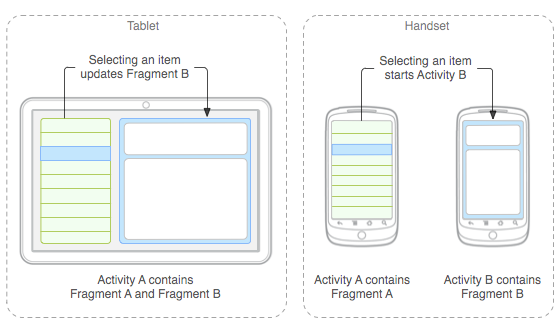
\includegraphics[scale=0.4]{chapters/ch11/images/1}
\end{center}

Ok, enough theory. Let's start coding and see how fragments are actually made.

\section{Create New Project}
\label{FRAG:createProj}

Create a new project from scratch. Perform the following steps:
\begin{enumerate}
	\item Create a new project having name ``\texttt{Fragments}''
	\item Select minimum API 16 : Android 4.1 (Jelly Bean).
	\item Select ``\texttt{Empty Activity}''
	\item Accept default values for activity and click finish. \\
\end{enumerate}

\section{Fragment Creation}
\label{FRAG:fragmentCreation}


